% Titre de la premiere partie
\section[]{My Progress}

%%%%%%%%%%%%%%%%%%%%%%%%%%%%%%%%%%%%%%%%%%%%%%%%
% Première diapo
%%%%%%%%%%%%%%%%%%%%%%%%%%%%%%%%%%%%%%%%%%%%%%%%
\begin{frame}
\frametitle{Toric Hyperk{\"a}hler Manifolds \& Compactification}
\framesubtitle{Hyperk{\"a}hler Analogues}

Complexification analogy for toric symplectic manifolds are \emph{hypertoric} manifolds: consider $M = T^{\ast}\CC^{n}$ with induced linear $G$-action from $\CC^{n}$, and moment map $\mu:\CC^{n} \rightarrow \mf{g}^{\ast}$.

Action is hyperhamiltonian with \HK moment map $\mu_{HK} := \mu_{\RR} \oplus \mu_{\CC}:T^{\ast}\CC^{n} \rightarrow \mf{g}^{\ast} \oplus \mf{g}_{\CC}^{\ast}$, where:
$$
	\mu_{\RR}(z,w) = \mu(z) - \mu(w),\qquad \mu_{\CC}(z,w)(v) =w(\hat{v}_{z}),
$$
with $w\in T_{z}^{\ast}\CC^{n}$, $v \in \mf{g}_{\CC}$, and $\hat{v}_{z} \in T_{z}\CC^{n}$ induced.
\begin{defn}
	For $\alpha \in Z(\mf{g}^{\ast})$:
	$$
		M := (\mu_{\RR}^{-1}(\alpha)\cap \mu_{\CC}^{-1}(0))/G
	$$
	is the \emph{hyperk{\"a}hler analogue} to the K{\"a}hler $X = \mu^{-1}(\alpha)/G$.
\end{defn}

\end{frame}

%%%%%%%%%%%%%%%%%%%%%%%%%%%%%%%%%%%%%%%%%%%%%%%%
% Première diapo
%%%%%%%%%%%%%%%%%%%%%%%%%%%%%%%%%%%%%%%%%%%%%%%%
\begin{frame}
	\frametitle{Toric Hyperk{\"a}hler Manifolds \& Compactification}
	\framesubtitle{Toric Hyperk{\"a}hler Manifolds}
	
	Let $X = \mu^{-1}(\alpha)/N$ be a symplectic toric manifold with a residual $T^{d} = T^{n}/N$ action from the Delzant construction.
	\begin{defn}
		A \emph{toric hyperk{\"a}hler manifold} $M$ is the hyperk{\"a}hler analogue to the K{\"a}hler quotient $X$.
	\end{defn}
	Explicitly:
	$$
		M = (\mu_{\RR}^{-1}(\alpha) \cap \mu_{\CC}^{-1}(0))/N,
	$$
	and, if $i^{\ast}(r_{1},\ldots, r_{n}) = \alpha$ and $(\partial_{i})_{i=1}^{n}$ is a basis for $(\RR^{d})^{\ast} = \ker i^{\ast}$, we get residual moment maps:
	$$
		\phi_{\RR}[z,w] = \frac{1}{2}\sum_{i=1}^{n}(|z_{i}|^{2} - |w_{i}|^{2} - r_{i})\partial_{i},\qquad \phi_{\CC}[z,w] = \sum_{i=1}^{n}(z_{i}w_{i})\partial_{i}.
	$$
\end{frame}

%%%%%%%%%%%%%%%%%%%%%%%%%%%%%%%%%%%%%%%%%%%%%%%%
% Première diapo
%%%%%%%%%%%%%%%%%%%%%%%%%%%%%%%%%%%%%%%%%%%%%%%%
\begin{frame}
	\frametitle{Toric Hyperk{\"a}hler Manifolds \& Compactification}
	\framesubtitle{The Extended Core}

\begin{defn}
	The set
	$$
		\mc{E} := \phi_{\CC}^{-1}(0) = \{[z,w] \in M \st z_{i}w_{i} = 0 \}
	$$
	is called the \emph{extended core} of $M$.
\end{defn}

For each $A \subseteq \{1,\ldots, n\}$, $\mc{E}$ breaks up into components:
$$
\mc{E}_{A} = \{[z,w] \in M \st w_{i} = 0 \text{ if } i \in A, \text{ and } z_{i} = 0 \not\in A   \},
$$ 
with image
$$
\Delta_{A} := \phi_{\RR}(\mc{E}_{A}) = \bigcap_{i \in A}F_{i} \cap \bigcap_{i\not\in A} G_{i}, 
$$
for
$$
	F_{i} = \{y \in (\RR^{d})^{\ast}\st \langle y, u_{i}\rangle + r_{i} \geq 0 \},\quad G_{i} = \{y \in (\RR^{d})^{\ast}\st \langle y,u_{i}\rangle + r_{i} \leq 0 \}.
$$

\end{frame}

%%%%%%%%%%%%%%%%%%%%%%%%%%%%%%%%%%%%%%%%%%%%%%%%
% Première diapo
%%%%%%%%%%%%%%%%%%%%%%%%%%%%%%%%%%%%%%%%%%%%%%%%
\begin{frame}
	\frametitle{Toric Hyperk{\"a}hler Manifolds \& Compactification}
	\framesubtitle{Example, $T^{\ast}\CC\PP^{2}$}

	\begin{figure}
		\centering
		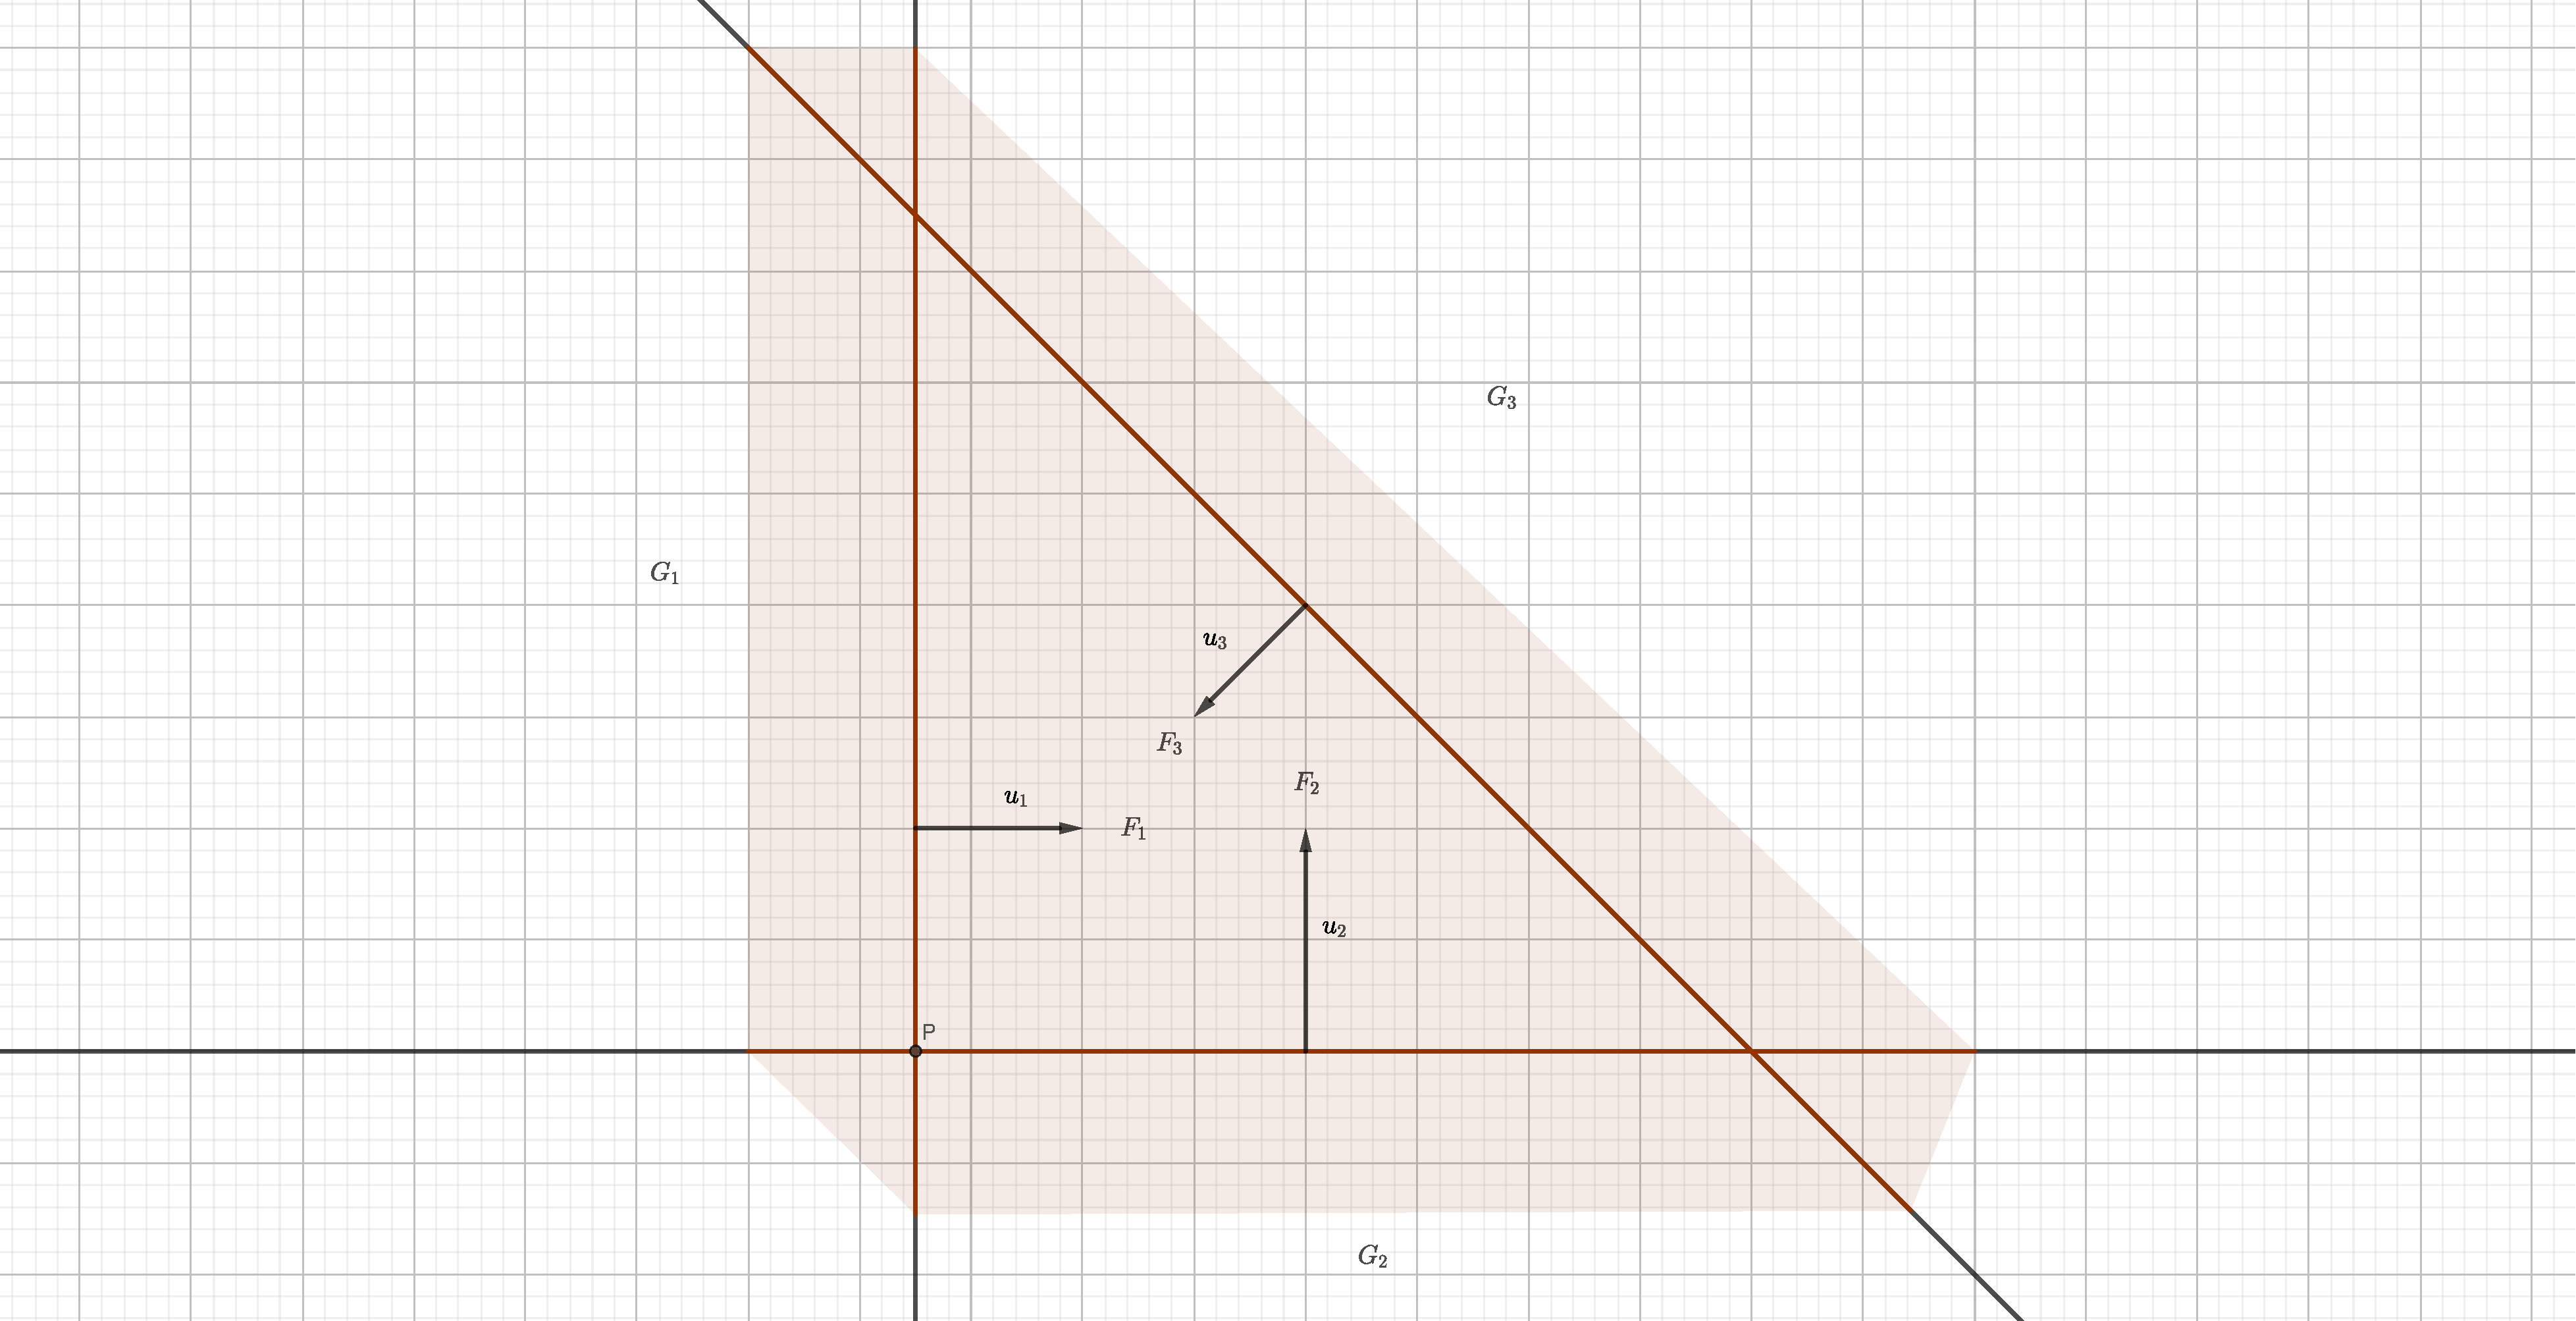
\includegraphics[width=1.2\linewidth]{figures/cp2-components}
	\end{figure}

\end{frame}

%%%%%%%%%%%%%%%%%%%%%%%%%%%%%%%%%%%%%%%%%%%%%%%%
% Première diapo
%%%%%%%%%%%%%%%%%%%%%%%%%%%%%%%%%%%%%%%%%%%%%%%%
\begin{frame}
	\frametitle{Toric Hyperk{\"a}hler Manifolds \& Compactification}
	\framesubtitle{Residual Circle Action}
	$$
		S^{1}\text{-action:}\qquad\hbar\cdot [z,w] = [z,\hbar w],\qquad \hbar \in S^{1}.
	$$
	Descends to $\mc{E}$ and, on each $\mc{E}_{A}$, acts as a subgroup of $T^{n}$. On $\mc{E}_{A}$:
	$$
		[z,\hbar w] = [\hbar^{-1}z_{1}, \ldots, \hbar^{-1}z_{n}; w] = [\hbar_{1}z_{1},\ldots, \hbar_{n}z_{n}; w],
	$$
	with
	$$
	\hbar_{i} :=
		\begin{cases}
		\hbar^{-1},\quad &\text{if } i \in A,\\
		1,\quad &\text{if } i \not\in A.
		\end{cases}
	$$
	For $j_{A}:\restr{S^{1}}{\mc{E}_{A}} \hookrightarrow T^{n}$, its moment map is
	$$
		\Phi_{A}[z,w] = -\bigg\langle \mu_{\RR}[z,w], \sum_{i\in A} u_{i} \bigg\rangle.
	$$
\end{frame}

%%%%%%%%%%%%%%%%%%%%%%%%%%%%%%%%%%%%%%%%%%%%%%%%
% Première diapo
%%%%%%%%%%%%%%%%%%%%%%%%%%%%%%%%%%%%%%%%%%%%%%%%
\begin{frame}
	\frametitle{Toric Hyperk{\"a}hler Manifolds \& Compactification}
	\framesubtitle{Compactification via Symplectic Cutting}
	
	Globally $\Phi[z,w] = \tfrac{1}{2}\|w\|^{2}$ is proper; can ``compactify'' $M$: let $S^{1}$ act on $M \times \CC$ diagonally. Moment map:
	$$
		\mu_{\text{cut}}:M \times \CC \rightarrow \RR,\qquad ([z,w],\xi) \mapsto \Phi[z,w] + \tfrac{1}{2}|\xi|^{2}.
	$$
	Resulting in:
	$$
	M_{\epsilon} := \mu_{\text{cut}}^{-1}(\epsilon)/S^{1} \cong \{m\in M \st \Phi(m) < \epsilon \} \sqcup \Phi^{-1}(\epsilon)/S^{1}
	$$
	On each component $\mc{E}_{A}^{(\epsilon)} := \mc{E}_{A} \cap M_{\epsilon}$, we find that:
	$$
		\phi_{\RR}(\mc{E}_{A}^{(\epsilon)}) = \Delta_{A} \cap \{ v \in (\RR^{d})^{\ast} \st \langle v, {\scriptstyle\sum}_{i\in A} u_{i} \rangle \leq \e   \}
	$$
\end{frame}

%%%%%%%%%%%%%%%%%%%%%%%%%%%%%%%%%%%%%%%%%%%%%%%%
% Première diapo
%%%%%%%%%%%%%%%%%%%%%%%%%%%%%%%%%%%%%%%%%%%%%%%%
\begin{frame}
	\frametitle{Toric Hyperk{\"a}hler Manifolds \& Compactification}
	\framesubtitle{Example for $T^{\ast}\CC\PP^{2}$}
	
	\begin{figure}
		\centering
		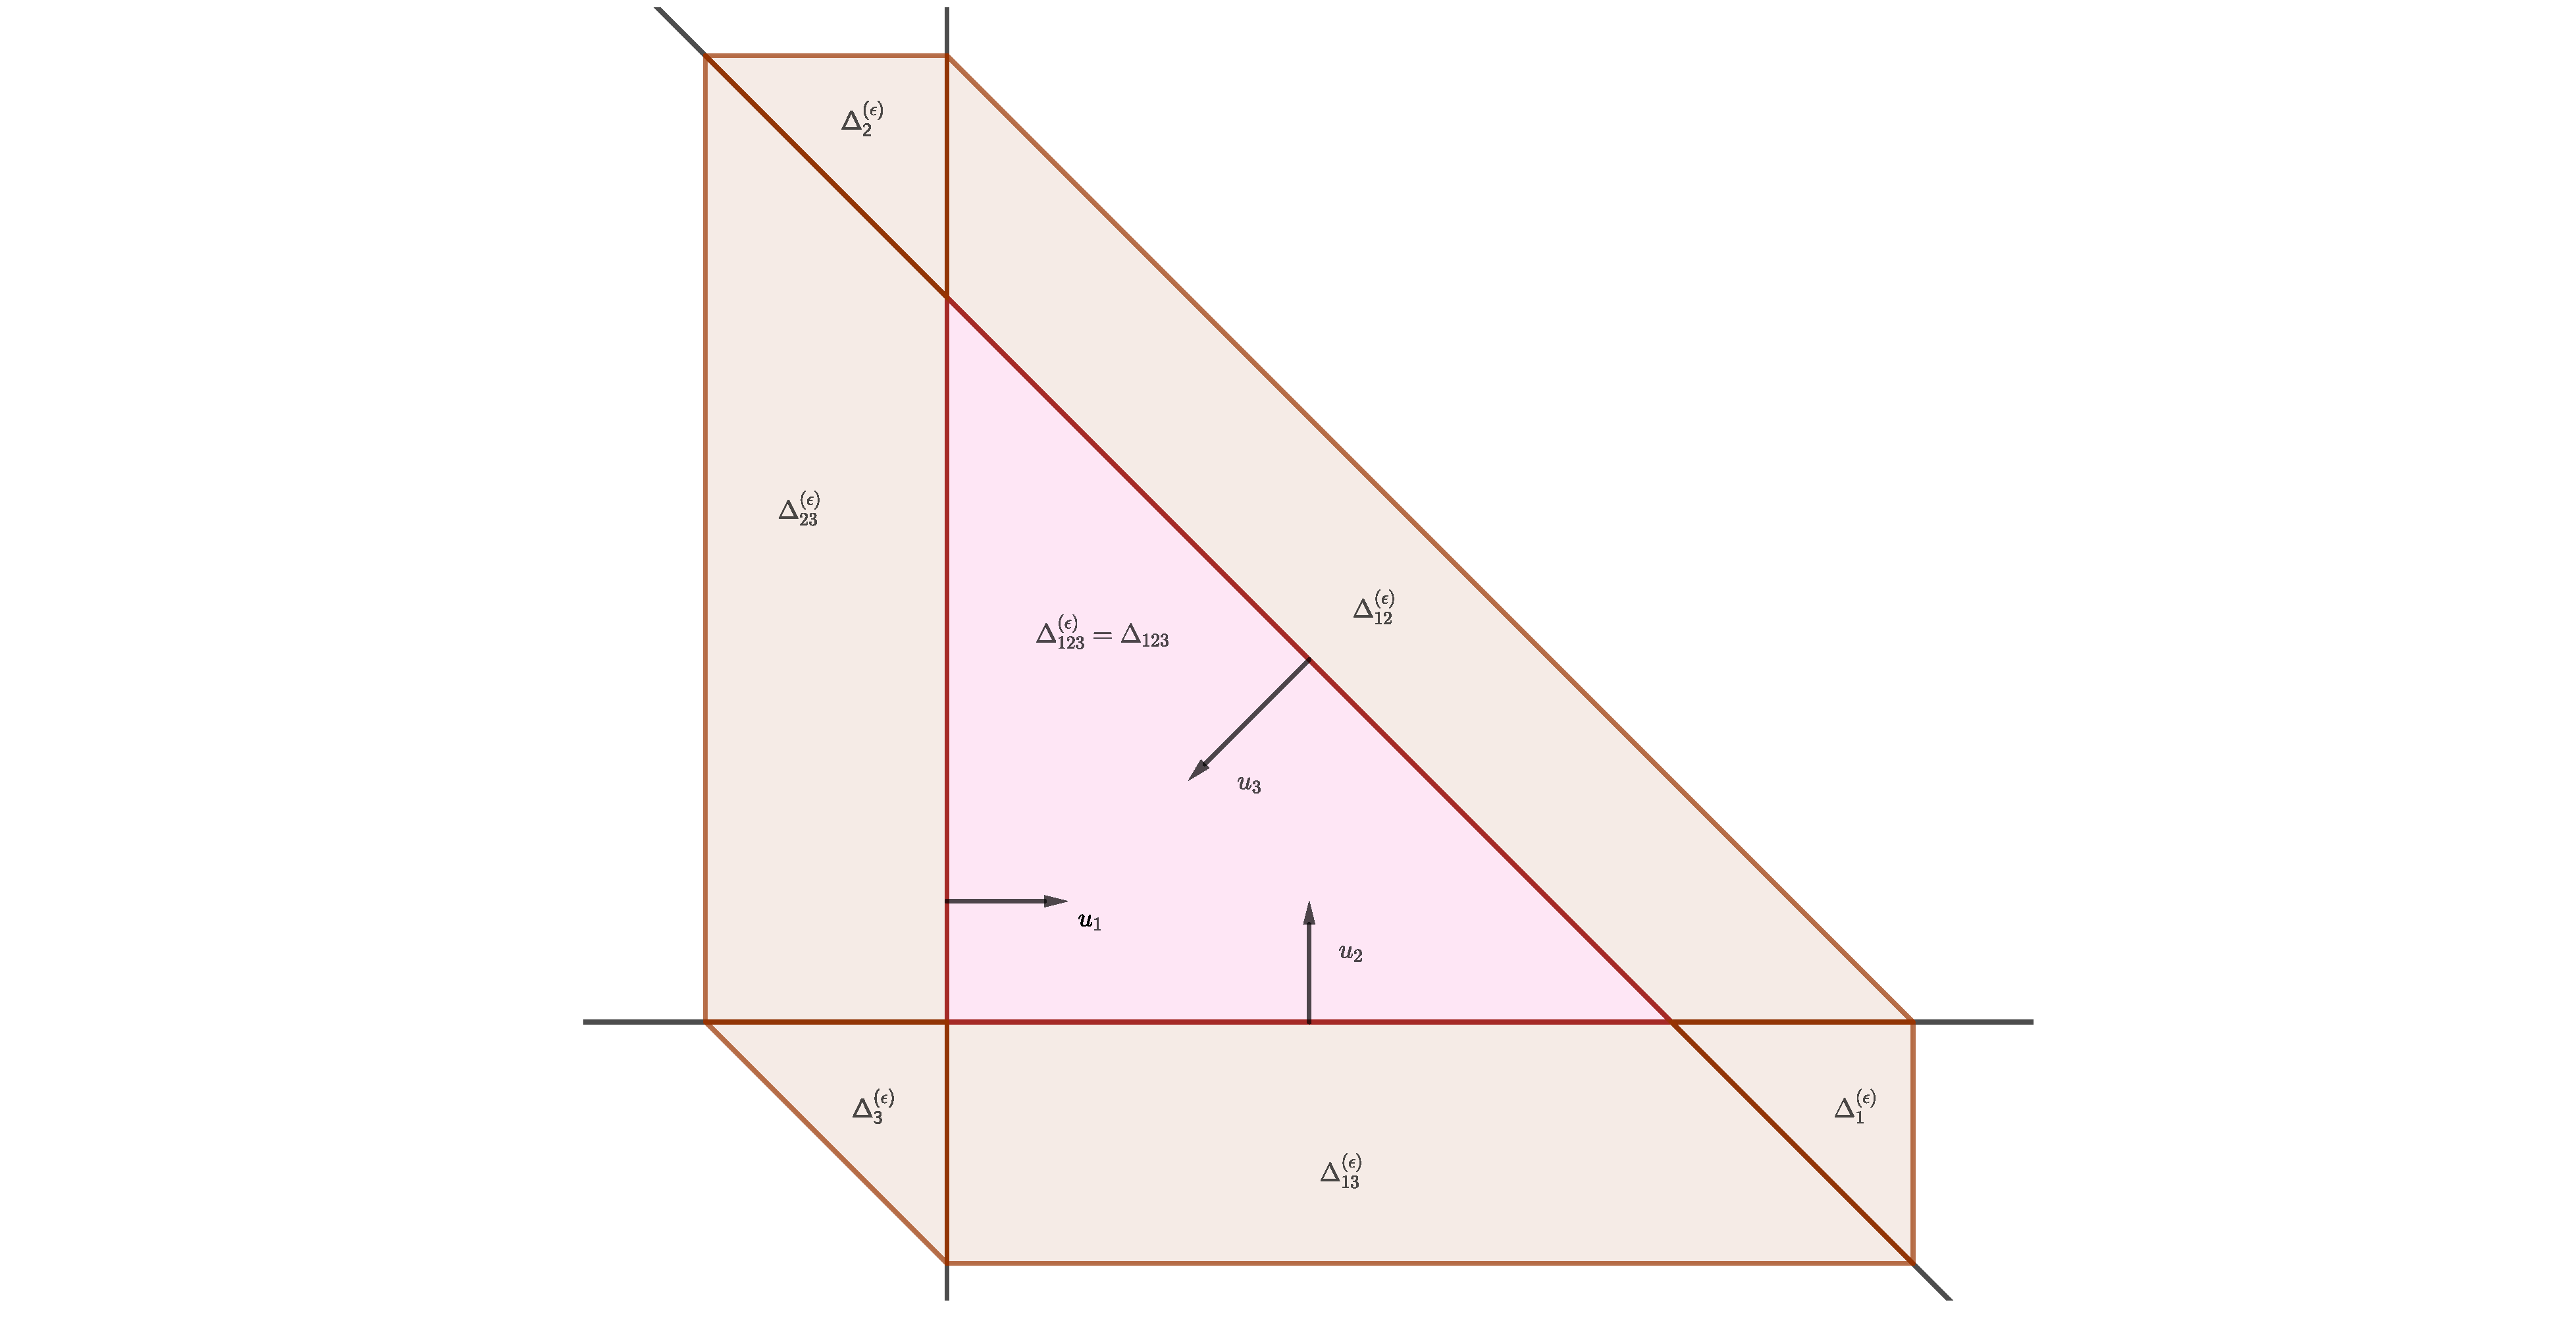
\includegraphics[width=0.7\linewidth]{figures/Symplectic_Cut_Cotangent_CP2}
	\end{figure}

\end{frame}

%%%%%%%%%%%%%%%%%%%%%%%%%%%%%%%%%%%%%%%%%%%%%%%%
% Première diapo
%%%%%%%%%%%%%%%%%%%%%%%%%%%%%%%%%%%%%%%%%%%%%%%%
\begin{frame}
	\frametitle{Toric Hyperk{\"a}hler Manifolds \& Compactification}
	\framesubtitle{Example for $T^{\ast}\CC\PP^{3}$}
	
	\begin{figure}
		\centering
		\begin{subfigure}{.5\textwidth}
			\centering
			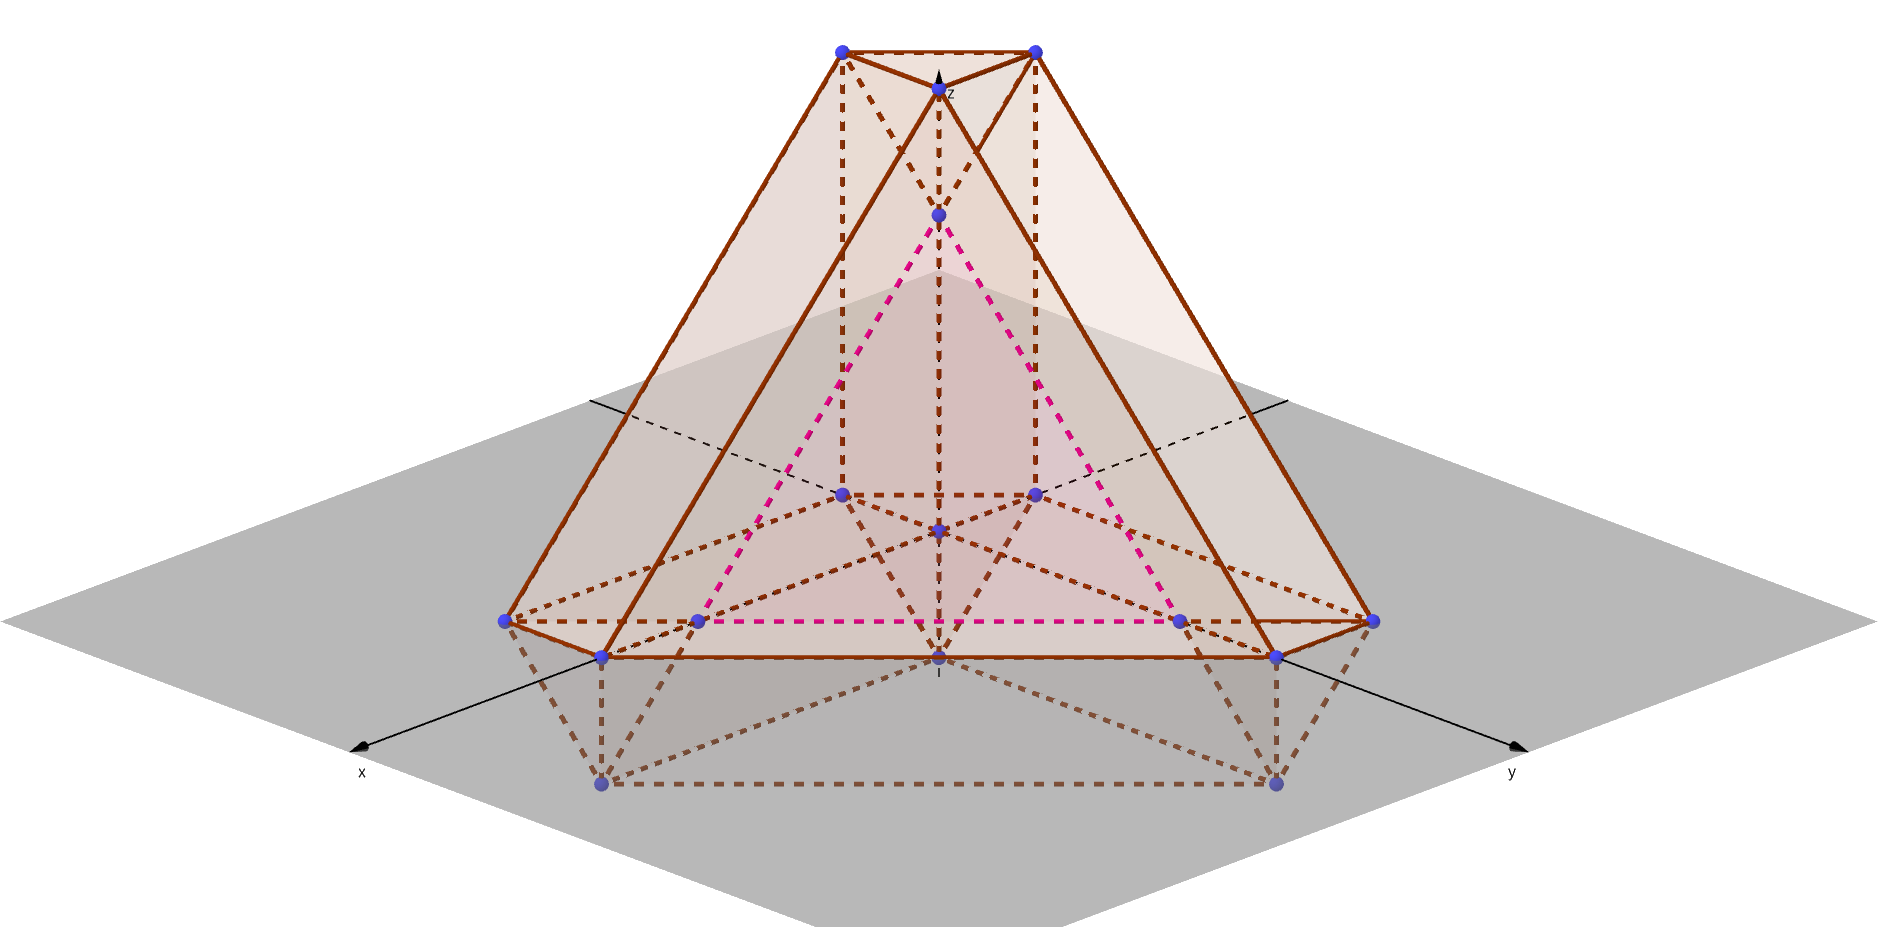
\includegraphics[width=1.2\linewidth]{figures/Symplectic_Cut_Cotangent_CP3.png}
		\end{subfigure}%
		\begin{subfigure}{.5\textwidth}
			\centering
			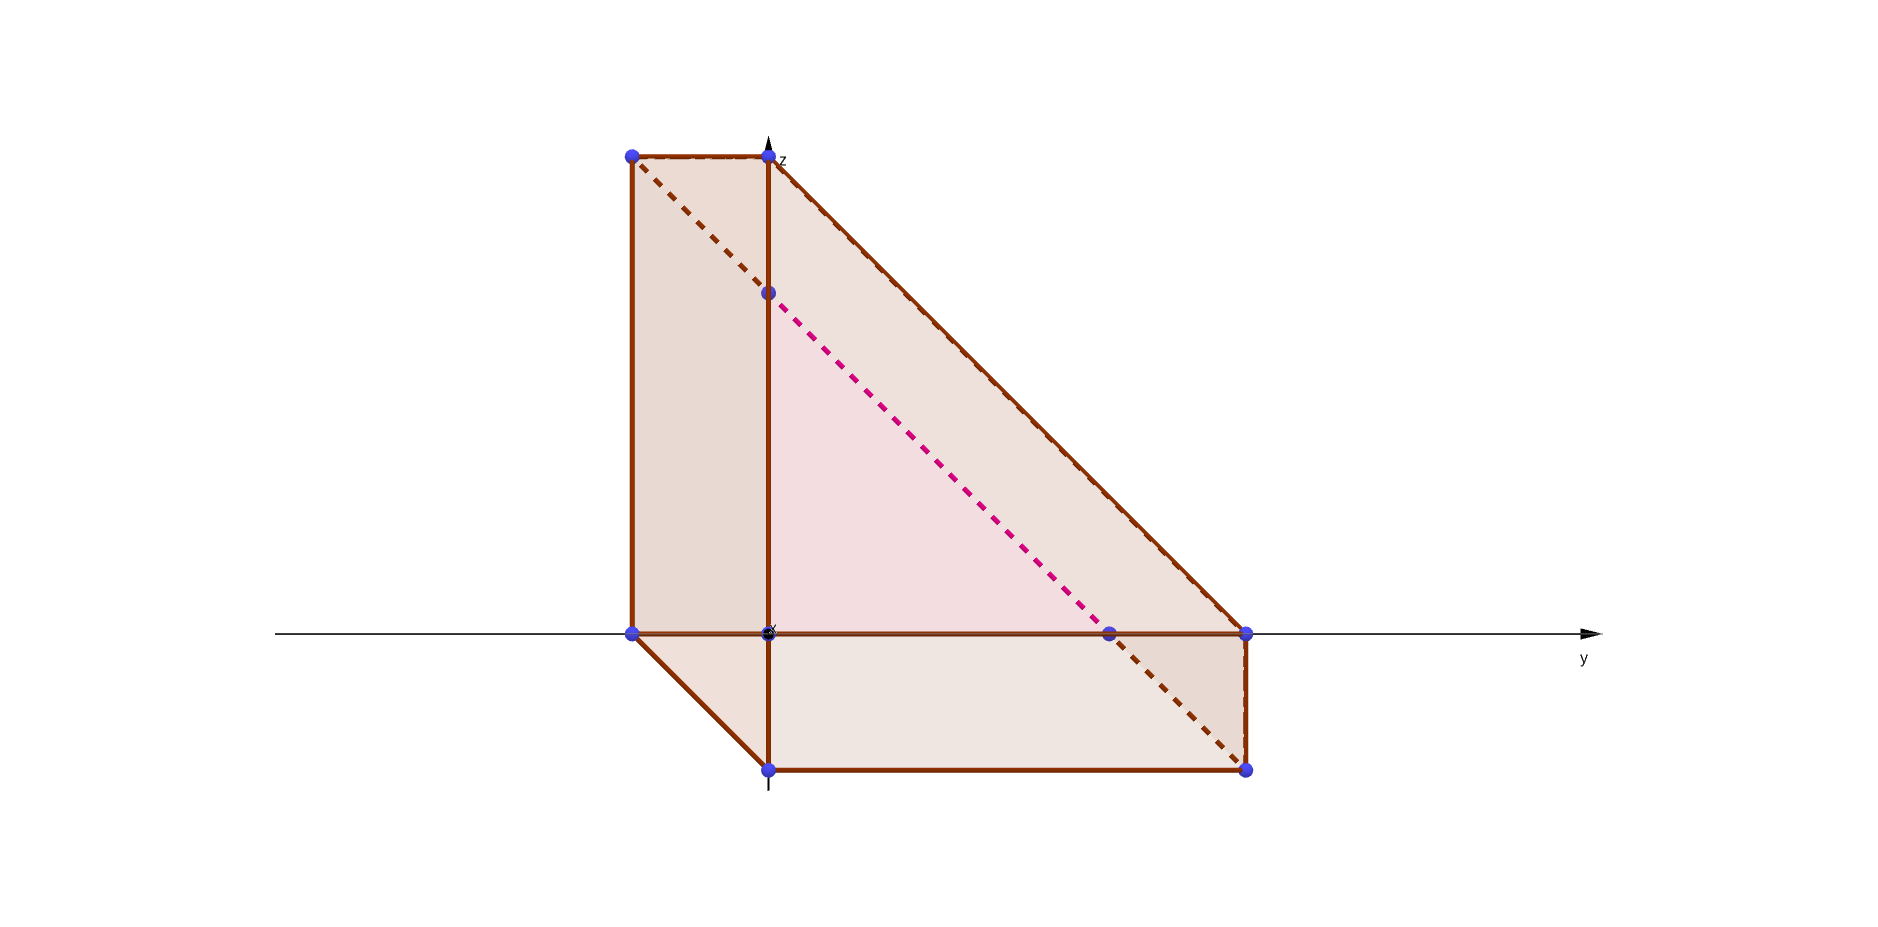
\includegraphics[width=1.2\linewidth]{figures/Symplectic_Cut_Cotangent_CP3-side.png}
		\end{subfigure}
	\end{figure}
	
	
\end{frame}


